% Copyright 2018 Sebastian B. Galkin

% This file is part of paraseba/scaladores-may-2018-talk.

% paraseba/scaladores-may-2018-talk is free software: you can redistribute it and/or modify
% it under the terms of the GNU General Public License as published by
% the Free Software Foundation, either version 3 of the License, or
% (at your option) any later version.

% paraseba/scaladores-may-2018-talk is distributed in the hope that it will be useful,
% but WITHOUT ANY WARRANTY; without even the implied warranty of
% MERCHANTABILITY or FITNESS FOR A PARTICULAR PURPOSE.  See the
% GNU General Public License for more details.

% You should have received a copy of the GNU General Public License
% along with Foobar.  If not, see <http://www.gnu.org/licenses/>.




% Title: Monoid driven design
% Titulo: Desenho dirigido por monoides

% Abstract:
% We will learn about Monoids, a concept invented (discovered?) by mathematicians
% that we can leverage to great value in our code and designs.

% The talk is structured in two sessions, in this first one (5/29) we'll learn what
% Monoids are, go through many examples, and write code that creates and uses Monoids. In
% the second session (June maybe?) we will see how we can use Monoids to guide software design.

% Despite the weird name, Monoids are easy to understand, and once you do, you'll
% start finding them everywhere. More importantly, after a little practice
% you'll gain intuition and you'll be able to integrate Monoids in your code and
% designs, obtaining more abstract and reusable results.

% Requirements:
% This is an intermediate level talk. No knowledge of math or functional
% programming is required. I'll assume you can understand simple Scala code.
% In particular, if you don't know what implicit parameters are, spend 10 minutes
% learning about them. You don't need to understand the details of implicit search
% mechanisms or anything like that.


% Resumo:
% Na primeira parte da palestra (https://www.youtube.com/watch?v=z2N-g6iSJJc)
% descubrimos os monoides e vimos varios exemplos de como usa-los na programacao.
% Nesta segunda parte vamos ver em profundidade um exemplo de como os monoides podem nos
% guiar en el desenho do nosso sistema.
%

% Requerimentos:
% Para aproveitar a palestra ao maximo, os participantes deveriam saber o que eh
% um monoide, eh exemplos basicos de monoides utis. Recomendo assistir a
% primeira parte de palestra onde poderam encontrar todas as informacoes
% necessarias:
% youtube: https://www.youtube.com/watch?v=z2N-g6iSJJc)
% slides: https://github.com/paraseba/scaladores-may-2018-talk


% Bio:

% Depois de quase uma década trabalhando em linguagens imperativas, Sebastian
% abraçou a programação funcional e nunca mais olhou para atrás. Nos últimos oito anos
% ele tem trabalhado nas áreas de data science, infraestrutura de Big Data e
% enterprise software, em linguagens como Scala, Haskell e Clojure. Cuidado!
% O Sebastian vai tentar trazer você para o mundo da programação funcional.


\documentclass{beamer}
\usepackage[english]{babel}
\usepackage[utf8]{inputenc}
\usepackage[T1]{fontenc}
\usepackage{pgfpages}
\usepackage{listings}
\usepackage{color}
\usepackage{ulem} % for \sout
\usepackage{tikz}
\usepackage{amsmath}
\usepackage{upquote} % make verbatin quotes vertical
\usepackage{adjustbox}

\usetikzlibrary{arrows,positioning,shapes,fit,calc}
\pgfdeclarelayer{background}
\pgfsetlayers{background,main}

\mode<presentation>
{
  \usetheme{Madrid}      % or try Darmstadt, Madrid, Warsaw, ...
  \usecolortheme{default} % or try albatross, beaver, crane, ...
  \usefonttheme{default}  % or try serif, structurebold, ...
  \useoutertheme{default}
  \setbeamertemplate{navigation symbols}{}
  \setbeamertemplate{caption}{\tiny\insertcaption\par}
  \setbeamertemplate{footline}{}

  % \AtBeginSection[]
  % {
  %   \begin{frame}<beamer>\frametitle{OUTLINE}
  %     \tableofcontents[currentsection,currentsection]
  %   \end{frame}
  % }

}

%\setbeameroption{show notes on second screen}
%\setbeameroption{show only notes}

\setbeamerfont{note page}{size=\tiny}
\setbeamertemplate{note page}[plain]


\adjustboxset{cfbox=blue {\fboxrule} 3ex, center}


\title[Monoids]{DESIGNING WITH MONOIDS}
\author{Sebastian Galkin}
\institute[@paraseba]{\texttt{@paraseba} \\ \texttt{paraseba@gmail.com}}
\date[Scaladores]{Scaladores - Nov 2018}
\subject{Talks}

\begin{document}
\lstset{
  language=Scala,
  basicstyle={\small\ttfamily},
  keywordstyle={\usebeamercolor{example text}\color{fg}},
  commentstyle={\usebeamercolor{palette sidebar tertiary}\color{fg!170!}\itshape},
  columns=fullflexible,
  keepspaces=true,
  escapechar=~,
  showlines=false,
}


\begin{frame}
  \titlepage
  \vspace{1cm}
  \begin{block}{}
    \centering
    \large{Ask questions as we go.}
  \end{block}
\end{frame}

\begin{frame}[plain]
  \center
\includegraphics[keepaspectratio=true,width=0.45\paperwidth]{brain.jpg}
\end{frame}


{
\usebackgroundtemplate{\includegraphics[width=\paperwidth]{papers.jpg}}
\begin{frame}[plain]
  \begin{block}{}

  Brent A. Yorgey,

  {\it \bf ``Monoids: Theme and Variations (Functional Perl)''}.

  July 2012.

  \end{block}
\end{frame}
}

\begin{frame}[fragile] \frametitle{PREREQUISITES}

  \begin{block}{Semigroup and Monoid}
  \begin{lstlisting}
trait Semigroup[M] {
  // moved from Monoid to its own class
  def ~\alert{append}~(a: M, b: => M): M
}

trait Monoid[A] extends Semigroup[M] {
  def ~\alert{zero}~: A
}

object SemigroupSyntax {
  final class SemigroupOps[A:Semigroup](val self: A) {
    def ~\alert{|+|}~(other: => A): A =
      Semigroup[A].append(self, other)
  }
  \end{lstlisting}
  \end{block}
\end{frame}

\begin{frame}[fragile] \frametitle{PREREQUISITES}
  \begin{block}{The Laws}
      \begin{itemize}
        \tt
        \item (a |+| b) |+| c === a |+| (b |+| c)
        \item a |+| zero === zero |+| a === a
      \end{itemize}
  \end{block}

  \begin{block}{The Canonical Examples}

  \begin{columns}
    \column{0.4\textwidth}
      \begin{itemize}
        \tt
      \item (Int, +, 0)
      \item (Int, *, 1)
      \end{itemize}
    \column{0.6\textwidth}
      \begin{itemize}
        \tt
      \item (List[A], ++, [])
      \item (A => A, andThen, identity)
      \end{itemize}
  \end{columns}
  \end{block}

  \begin{block}{Using \texttt{Monoids}}
  \begin{lstlisting}
implicit val intSumMon: Monoid[Int] = ....
implicit def listMon[A]: Monoid[List[A]] = ....

val five = 3 |+| 2
val l = List(1,2,3) |+| List(4,5,6)
  \end{lstlisting}
  \vspace{-.5cm}
  \end{block}
\end{frame}

\begin{frame}[fragile] \frametitle{REFRESHER ON WRITING MONOIDS}
  \begin{block}{Writing a \texttt{List Monoid}}
  \begin{lstlisting}
implicit def listMon[A]: Monoid[List[A]] = new Monoid[List[A]] {
  def append(as: List[A], bs: => List[A]): List[A] =
    as ++ bs

  def zero: List[A] = List()
}
  \end{lstlisting}
  \vspace{-.5cm}
  \end{block}

  \vspace{-.1cm}

  \begin{block}{The All-Purpose Function: \texttt{mconcat}}
  \begin{lstlisting}
// mconcat(List(a1,a2,a3,...)) === a1 |+| a2 |+| a3 |+| ...
def mconcat[A:Monoid](as: Traversable[A]): A =
  as.foldLeft(Monoid[A].zero)(_ |+| _)

val five = mconcat(List(0,1,2,2))(intAddMonoid)
  \end{lstlisting}
  \vspace{-.5cm}
  \end{block}

  \vspace{-.1cm}

  \begin{block}{}
    \centering
    \bf
    Any doubts about monoids?
  \end{block}

\end{frame}

\begin{frame}[fragile] \frametitle{DIAGRAM 1.0 --- A LIST OF PRIMITIVES}
  \begin{block}{A Diagram as a List of Primitives}
  \begin{lstlisting}
sealed trait Prim { def draw(...) ... }

final case class Point(x: Double,
                       y: Double,
                       c: Color, ...) extends Prim

final case class Line(...) extends Prim
final case class Ellipse(...) extends Prim
... ~\pause~

// Let's say the primitives are drawn in the list order
final case class Diagram(primitives: List[Prim])
  \end{lstlisting}
  \end{block}

  How do \texttt{Diagrams} combine (or compose)?
\end{frame}

\begin{frame}[fragile] \frametitle{DIAGRAM 1.0 --- A LIST OF PRIMITIVES}
Diagrams compose by drawing them on top of each other.
  \begin{block}{The Diagram Monoid}
  \begin{lstlisting}
object Diagram {

  val diagramMonoid = new Monoid[Diagram] {
    def zero: Diagram = Diagram(listMon.zero)

    def append(d1: Diagram, d2: => Diagram): Diagram =
      Diagram(listMon.append(d1.primitives, d2.primitives))
  }
}
  \end{lstlisting}
  \end{block}
\end{frame}

\begin{frame}[fragile] \frametitle{DIAGRAM 1.0 --- A LIST OF PRIMITIVES}
  \begin{block}{Helper for Wrapped Monoids}
  \begin{lstlisting}
def wSemi[Out, ~\alert{In:Semigroup}~](un: Out => In,
                             wr: In => Out): Semigroup[Out] = ~\pause~
  new Semigroup[Out] {
    def append(x:Out, y: => Out) = wr(un(x) |+| un(y))
  } ~\pause~

def wMon[Out, In:Monoid](un: Out => In,
                         wr: In => Out): Monoid[Out] =
  new Monoid[Out] {
    def append(x: Out, y: => Out) = wr(un(x) |+| un(y))
    def zero = wr(implicitly[Monoid[In]].zero)
  }
  \end{lstlisting}
  \end{block}
Using the implicit \texttt{Monoid} instance.
\end{frame}

\begin{frame}[fragile] \frametitle{DIAGRAM 1.0 --- A LIST OF PRIMITIVES}
  \begin{block}{The Diagram Monoid}
  \begin{lstlisting}
// remember the definition of Diagram
final case class Diagram(primitives: List[Prim])

object Diagram {

  val diagramMonoid: ~\alert{Monoid[Diagram]}~ =
    wMon(_.primitives, Diagram(_))
}
  \end{lstlisting}
  \end{block}

  And now we can combine \texttt{Diagrams} drawing one on top of the other.

  But we would want \alert{\texttt{d1 |+| d2} to draw \texttt{d1} on top.}
\end{frame}

\begin{frame}[fragile] \frametitle{DIAGRAM 1.0 --- A LIST OF PRIMITIVES}
  \begin{block}{Fixing the Order}
  \begin{lstlisting}
final case class Dual[M](undual: M)

implicit def dualMonoid[M:Monoid] = new Monoid[Dual[M]] {
  def zero = Dual(implicitly[Monoid[M]].zero)

  def append(a: Dual[M], b : => Dual[M]) =
    Dual(~\alert{b}~.undual |+| ~\alert{a}~.undual)
} ~\pause~

final case class Diagram(primitives: Dual[List[Prim]])

object Diagram {
  val diaMon: Monoid[Diagram] = wMon(_.primitives, Diagram(_))
}
  \end{lstlisting}
    \vspace{-0.3cm}
  \end{block}

Look how expressive the type for \texttt{Diagram} is!
\end{frame}

\begin{frame}[fragile] \frametitle{DIAGRAM 2.0 --- BESIDE}
A different way to compose \texttt{Diagrams}.

  \begin{figure}
      \centering
      \adjustbox{}{
        \includegraphics[width=0.25\textwidth]{beside.png}
      }
      \caption{Monoids: Theme and Variations (Functional Perl)}
  \end{figure}

\vspace{-0.5cm}

  \begin{block}{The \texttt{beside} Function}
    \vspace{-0.2cm}
  \begin{lstlisting}
// vectors on the plane
type V2 = (Double, Double)

def beside(v: V2, d1: Diagram, d2: Diagram): Diagram = ???
  \end{lstlisting}
\vspace{-0.5cm}
  \end{block}
\end{frame}

\begin{frame}[fragile] \frametitle{DIAGRAM 2.0 --- BESIDE}
  \begin{figure}
      \centering
      \adjustbox{}{
        \includegraphics[width=0.4\textwidth]{envelope.png}
      }
      \caption{Monoids: Theme and Variations (Functional Perl)}
  \end{figure}

  \vspace{-0.5cm}
  \pause

  \begin{block}{\texttt{Envelopes}: Function as Data}
  \begin{lstlisting}
final case class Envelope(f: V2 => Double)

def envelopeP(p: Prim): Envelope = ...
  \end{lstlisting}
  \end{block}
\end{frame}

\begin{frame} \frametitle{DIAGRAM 2.0 --- BESIDE}
  \begin{figure}
      \centering
      \adjustbox{}{
        \includegraphics[width=0.5\textwidth]{composeenv.png}
      }
      \caption{Monoids: Theme and Variations (Functional Perl)}
  \end{figure}

  \texttt{Envelopes} compose by taking the maximum distance in every direction.
\end{frame}


\begin{frame}[fragile] \frametitle{DIAGRAM 2.0 --- BESIDE}
  \begin{block}{Reminder: Functions that return a \texttt{Semigroup}}
  \begin{lstlisting}
implicit def funSemi[A, B:Semigroup]: Semigroup[A => B] =
  new Semigroup[A => B] {

    def append(f: A => B, g: => (A => B)): A => B =
      a => f(a) |+| g(a)
}
  \end{lstlisting}
  \end{block}

  We can use this for our

  \texttt{final case class Envelope(f: V2 => Double)}
\end{frame}

\begin{frame}[fragile] \frametitle{DIAGRAM 2.0 --- BESIDE}
  \begin{block}{A \texttt{Semigroup} for \texttt{Envelopes}}
  \begin{lstlisting}
// libraries provide this type out of the box
final case class Max[A](unmax: A)

implicit def maxSemi[A:Ordering] = new Semigroup[Max[A]] {
  def append(a: Max[A], b: => Max[A]): Max[A] =
    Max(Ordering[A].max(a.unmax, b.unmax))
} ~\pause~

// final case class Envelope(f: V2 => Double)
final case class Envelope(f: V2 => ~\alert{Max}~[Double])

val semiGroup: Semigroup[Envelope] = wSemi(_.f, Envelope(_))
  \end{lstlisting}
  \end{block}

  But we push for a \texttt{Monoid} for \texttt{Envelope}.
\end{frame}

\begin{frame}[fragile] \frametitle{DIAGRAM 2.0 --- BESIDE}
  \begin{block}{Reminder: \texttt{Option Monoid}}
  \begin{lstlisting}
// libraries provide this type out of the box
implicit def optionMon[A:Semigroup] = new Monoid[Option[A]] {
    def zero: Option[A] = None
    def append(a: Option[A], b: => Option[A]): Option[A] =
      (a,b) match {
        case (a, None) => a
        case (None, b) => b
        case (Some(a), Some(b)) => Some(a |+| b)
      }
}
  \end{lstlisting}
  \end{block}
\end{frame}

\begin{frame}[fragile] \frametitle{DIAGRAM 2.0 --- BESIDE}
  \begin{block}{A \texttt{Monoid} for \texttt{Envelopes}}
  \begin{lstlisting}
final case class Envelope(f: ~\alert{Option}~[V2 => Max[Double]])

val envMonoid: Monoid[Envelope] = wMon(_.f, Envelope(_))
  \end{lstlisting}
  \end{block}

Again, full expressiveness for \texttt{Envelope} type!
\end{frame}

\begin{frame} \frametitle{DIAGRAM 2.0 --- BESIDE}
Now we can write \texttt{beside}
  \begin{figure}
      \centering
      \adjustbox{}{
        \includegraphics[width=0.3\textwidth]{beside.png}
      }
      \caption{Monoids: Theme and Variations (Functional Perl)}
  \end{figure}
  \vspace{-.5cm}
  Translate the square in the direction \texttt{v} by:

  (Distance to the end of the circle in the direction \texttt{v}) +

  (Distance to the end of the square in the direction \texttt{-v})
\end{frame}

\begin{frame}[fragile] \frametitle{DIAGRAM 2.0 --- BESIDE}
  \begin{block}{\texttt{beside} Is Just Composition of Translated Diagrams}
  \begin{lstlisting}
def beside(v: V2, d1: Diagram, d2: Diagram): Diagram =
  (envelope(d1).f, envelope(d2).f) match {

    case (Some(f1), Some(f2)) =>
      d1 |+| translate(v * (f1(v).unmax + f2(-v).unmax), d2)

    case _ => d1 |+| d2
  }

// Monoid magic
def envelope(d: Diagram): Envelope =
  mconcat(d.primitives.undual.map(envelopeP))

def translate(v: V2, d: Diagram): Diagram =
  Diagram(Dual(d.primitives.undual.map(translateP(v, _))))
  \end{lstlisting}
  \vspace{-0.4cm}
  \end{block}
\end{frame}

\begin{frame} \frametitle{DIAGRAM 3.0 --- TRACES}
How to draw a ray between diagrams?

  \begin{figure}
      \centering
      \adjustbox{}{
        \includegraphics[width=0.9\textwidth]{tracevsenv.png}
      }
      \caption{Monoids: Theme and Variations (Functional Perl)}
  \end{figure}

Envelopes clearly don't work.
\end{frame}

\begin{frame}[fragile] \frametitle{DIAGRAM 3.0 --- TRACES}
  \begin{figure}
      \centering
      \adjustbox{}{
        \includegraphics[width=0.3\textwidth]{trace.png}
      }
      \caption{Monoids: Theme and Variations (Functional Perl)}
  \end{figure}

  \begin{block}{A \texttt{Trace} Is (Again) a Function}
  \begin{lstlisting}
// points on the plane
type P2 = (Double, Double)

final case class Trace(f: P2 => V2 => Double)
  \end{lstlisting}
  \vspace{-0.4cm}
  \end{block}
\end{frame}

\begin{frame}[fragile] \frametitle{DIAGRAM 3.0 --- TRACES}
  How do \texttt{Traces} compose?

  \begin{block}{A \texttt{Semigroup} for \texttt{Traces}}
  \begin{lstlisting}
// libraries provide this type out of the box
final case class Min[A](unmin: A)

implicit def minSemi[A:Ordering] = new Semigroup[Min[A]] {
  def append(a: Min[A], b: => Min[A]): Min[A] =
    Min(Ordering[A].min(a.unmin, b.unmin))
} ~\pause~

// final case class Trace(f: P2 => V2 => Double)
final case class Trace(f: P2 => V2 => ~\alert{Min}~[Double])

val semiGroup: Semigroup[Trace] = wSemi(_.f, Trace(_))
  \end{lstlisting}
  \end{block}
\end{frame}

\begin{frame}[fragile] \frametitle{DIAGRAM 3.0 --- TRACES}
  But we push for a \texttt{Monoid}, not just a \texttt{Semigroup}!

  \begin{block}{Which One Should We Use?}
  \begin{lstlisting}
// P2 => V2 => Min[Double]

Option[P2 =>        V2 => Min[Double]]
       P2 => Option[V2 => Min[Double]]
       P2 =>        V2 => Option[Min[Double]]
  \end{lstlisting}
  \end{block}
\end{frame}

\begin{frame}[fragile] \frametitle{DIAGRAM 3.0 --- TRACES}
  \begin{block}{The \texttt{Trace Monoid}}
  \begin{lstlisting}
final case class Trace(f: P2 => V2 => Option[Min[Double]])

def traceP(p: Prim): Trace = {...}

object Trace{
  implicit val traceMonoid: Monoid[Trace] = wMon(_.f, Trace(_))

  def trace(d: Diagram): Trace =
    mconcat(d.primitives.undual.map(traceP))
}
  \end{lstlisting}
  \end{block}

Again, full expressiveness for \texttt{Trace} type!
\end{frame}

\begin{frame}[fragile] \frametitle{DIAGRAM 4.0 --- CACHING}
  Computing \texttt{Envelopes} and \texttt{Traces} can become expensive.

  \begin{block}{Cached \texttt{Diagrams}}
  \begin{lstlisting}
final case class Diagram private (
  primitives: Dual[List[Prim]], env: Envelope, tr: Trace)

def envelope(d: Diagram): Envelope = d.env
def trace(d: Diagram): Trace = d.tr

def primDiag(p: Prim): Diagram =
  Diagram(Dual(List(p)), envelopeP(p), traceP(p))

object Diagram {
  def mkDiag(ps: List[Prim]): Diagram = mconcat(ps.map(primDiag))

  implicit val monoid: Monoid[Diagram] = wMon(..., ...)
}
  \end{lstlisting}
  \vspace{-.5cm}
  \end{block}
\end{frame}

\begin{frame}[fragile] \frametitle{DIAGRAM 4.0 --- CACHING}
  The only way to create composite diagrams is to use \texttt{|+|}

  \begin{block}{Complex \texttt{Diagrams}}
  \begin{lstlisting}
val d: Diagram = d1 |+| d2 |+| beside(v, d3, d4) |+| ...
  \end{lstlisting}
  \end{block}
  But will this work?

  \begin{block}{We Need to Verify}
  \begin{lstlisting}
def oldEnvelope(d: Diagram): Envelope =
  mconcat(d.primitives.undual.map(envelopeP))

oldEnvelope(Diagram(Dual(ps), e, t)) ==? e
  \end{lstlisting}
  \end{block}
\end{frame}



\begin{frame}[fragile] \frametitle{DIAGRAM 4.0 --- CACHING}
In pictures, the \texttt{oldEnvelope} function:

\begin{figure}
  \centering
  \begin{adjustbox}{}
    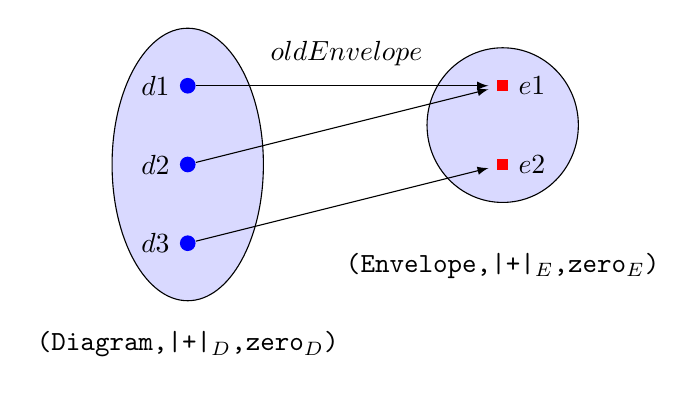
\begin{tikzpicture}[
      every node/.style={on grid},
      setA/.style={fill=blue,circle,inner sep=2pt},
      setB/.style={fill=red,rectangle,inner sep=2pt},
      every fit/.style={draw,fill=blue!15,ellipse,text width=32pt},
      >=latex
    ]

    % set A
    \node[setA,label=left:$d1$] (a) {};
    \node [setA,below = of a,label=left:$d2$] (b) {};
    \node [setA,below = of b,label=left:$d3$] (c) {};
    \node[below=of c,anchor=north] {\texttt{(Diagram,|+|$_D$,zero$_D$)}};

    % % set B
    \node[setB, right=4cm of a, label=right:$e1$] (x) {};
    \node[setB, below = of x, label=right:$e2$] (y) {};
    \node[below=of y,anchor=north] {\texttt{(Envelope,|+|$_E$,zero$_E$)}};

    % the arrows
    \draw[->,shorten >= 3pt] (a) -- node[label=above:$oldEnvelope$] {} (x);
    \draw[->,shorten >= 3pt] (b) -- node[] {} (x);
    \draw[->,shorten >= 3pt] (c) -- node[] {} (y);

    % the boxes around the sets
    \begin{pgfonlayer}{background}
    \node[fit= (a)  (c) ] {};
    \node[fit= (x) (y) ] {};
    \end{pgfonlayer}
    \end{tikzpicture}
  \end{adjustbox}
\end{figure}
\end{frame}

\begin{frame}[fragile] \frametitle{DIAGRAM 4.0 --- CACHING}
  \begin{block}{Proof}
\vspace{-.2cm}
  \begin{lstlisting}
oldEnvelope(zero~$_D$~)                                         ~\alert{$\longleftarrow$}~
zero~$_D$~ = mkDiag(List()) = Diagram(Dual(List.empty), zero~$_E$~, zero~$_T$~)
oldEnvelope(mkDiag(List())) = mconcat(List.empty) = zero~$_E$~  ~\alert{$\longleftarrow$} \pause~


oldEnvelope(d1 |+|~$_D$~ d2)  ~\alert{$\longleftarrow$}~
oldEnvelope(Diagram(Dual(p2 ++ p1), e1 |+|~$_E$~ e2, t1 |+|~$_T$~ t2))
= mconcat((p2 ++ p1).map(envelopeP))
= mconcat(p2.map(envelopeP) ++ p1.map(envelopeP))
= mconcat(p2.map(envelopeP)) |+|~$_E$~ mconcat(p1.map(envelopeP))
= oldEnvelope(d2) |+|~$_E$~ oldEnvelope(d1)
= oldEnvelope(d1) |+|~$_E$~ oldEnvelope(d2)
= e1 |+|~$_E$~ e2             ~\alert{$\longleftarrow$}~
  \end{lstlisting}
\vspace{-.4cm}
  \end{block}
\end{frame}

\begin{frame}[fragile] \frametitle{DIAGRAM 4.0 --- CACHING}
  As it turns out, \texttt{oldEnvelope} is a \texttt{Monoid} homomorphism.

\begin{figure}
  \centering
  \begin{adjustbox}{scale=0.8}
    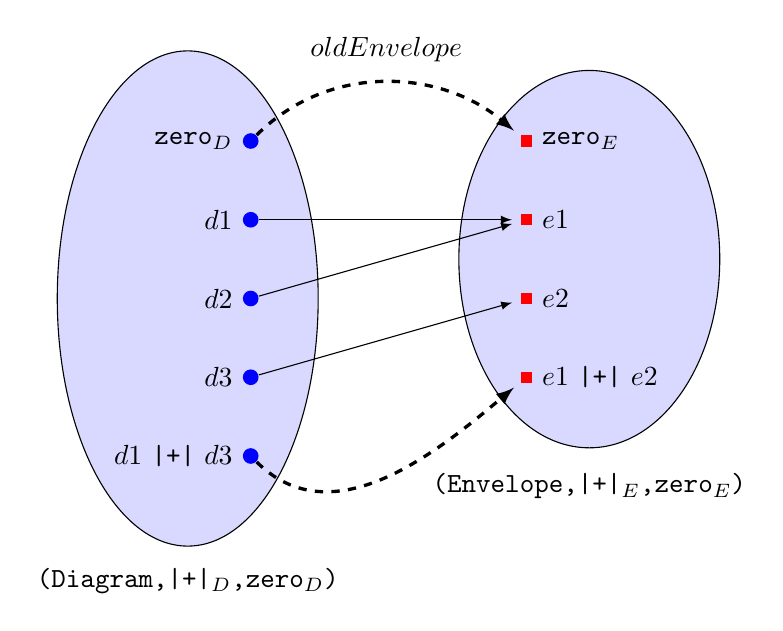
\begin{tikzpicture}[
      every node/.style={on grid},
      setA/.style={fill=blue,circle,inner sep=2pt},
      setB/.style={fill=red,rectangle,inner sep=2pt},
      every fit/.style={draw,fill=blue!15,ellipse,text width=60},
      >=latex
    ]

    % set A
    \node[setA,label=left:\texttt{zero}$_D$] (za) {};
    \node[setA,below = of za, label=left:$d1$] (a) {};
    \node [setA,below = of a,label=left:$d2$] (b) {};
    \node [setA,below = of b,label=left:$d3$] (c) {};
    \node [setA,below = of c,label=left:$d1$ \texttt{|+|} $d3$] (d) {};

    % % set B
    \node[setB,right=3.5cm of za, label=right:\texttt{zero}$_E$] (zb) {};
    \node[setB, below = of zb, label=right:$e1$] (x) {};
    \node[setB, below = of x, label=right:$e2$] (y) {};
    \node[setB, below = of y, label=right:$e1$ \texttt{|+|} $e2$] (z) {};

    % the arrows
    \draw[->,shorten >= 3pt, dashed, very thick] (za) to[out=45,in=140] node[label=above:$oldEnvelope$] {} (zb);
    \draw[->,shorten >= 3pt] (a) -- node[] {} (x);
    \draw[->,shorten >= 3pt] (b) -- node[] {} (x);
    \draw[->,shorten >= 3pt] (c) -- node[] {} (y);
    \draw[->,shorten >= 3pt, dashed, very thick] (d) to[out=-45,in=220] node[] {} (z);

    % the boxes around the sets
    \begin{pgfonlayer}{background}
      \node[fit= (za)  (d), shift={(-.8cm,0)} ] (ella) {};
      \node[fit= (zb) (z), shift={(.8cm,0)}  ] (ellb) {};
      \node[below=of ella,anchor=north,shift={(0,-2.3cm)}] {\texttt{(Diagram,|+|$_D$,zero$_D$)}};
      \node[below=of ellb,anchor=north,shift={(0,-1.6cm)}] {\texttt{(Envelope,|+|$_E$,zero$_E$)}};
    \end{pgfonlayer}
    \end{tikzpicture}
  \end{adjustbox}
\end{figure}
\end{frame}

\begin{frame}[fragile] \frametitle{DIAGRAM 4.0 --- CACHING}
A simpler example of a \texttt{Monoid} homomorphism.

\begin{figure}
  \centering

  \begin{adjustbox}{scale=0.8}
    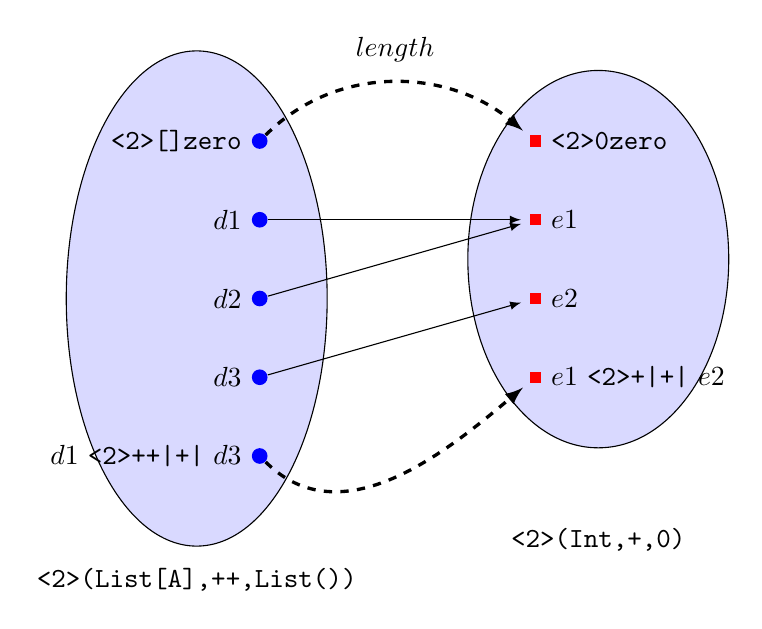
\begin{tikzpicture}[
      every node/.style={on grid},
      setA/.style={fill=blue,circle,inner sep=2pt},
      setB/.style={fill=red,rectangle,inner sep=2pt},
      every fit/.style={draw,fill=blue!15,ellipse,text width=60},
      >=latex
    ]

    % set A
    \node[setA,label=left:\texttt{\alt<2>{[]}{zero}}] (za) {};
    \node[setA,below = of za, label=left:$d1$] (a) {};
    \node [setA,below = of a,label=left:$d2$] (b) {};
    \node [setA,below = of b,label=left:$d3$] (c) {};
    \node [setA,below = of c,label=left:$d1$ \texttt{\alt<2>{++}{|+|}} $d3$] (d) {};

    % % set B
    \node[setB,right=3.5cm of za, label=right:\texttt{\alt<2>{0}{zero}}] (zb) {};
    \node[setB, below = of zb, label=right:$e1$] (x) {};
    \node[setB, below = of x, label=right:$e2$] (y) {};
    \node[setB, below = of y, label=right:$e1$ \texttt{\alt<2>{+}{|+|}} $e2$] (z) {};

    % the arrows
    \draw[->,shorten >= 3pt, dashed, very thick] (za) to[out=45,in=140] node[label=above:$length$] {} (zb);
    \draw[->,shorten >= 3pt] (a) -- node[] {} (x);
    \draw[->,shorten >= 3pt] (b) -- node[] {} (x);
    \draw[->,shorten >= 3pt] (c) -- node[] {} (y);
    \draw[->,shorten >= 3pt, dashed, very thick] (d) to[out=-45,in=220] node[] {} (z);

    % the boxes around the sets
    \begin{pgfonlayer}{background}
      \node[fit= (za)  (d), shift={(-.8cm,0)} ] (ella) {};
      \node[fit= (zb) (z), shift={(.8cm,0)}  ] (ellb) {};

      \node[below=of ella,anchor=north,shift={(0,-2.3cm)}] {\texttt{\uncover<2>{(List[A],++,List())}}};
      \node[below=of ellb,anchor=north,shift={(0,-2.3cm)}] {\texttt{\uncover<2>{(Int,+,0)}}};
    \end{pgfonlayer}
    \end{tikzpicture}
  \end{adjustbox}
\end{figure}
\end{frame}

\begin{frame} \frametitle{CONCLUSIONS}
  \begin{itemize}
    \item In many problems \alert{composition is the most important operation.}
    \item Try a \texttt{Monoid}/\texttt{Semigroup} as the means of composition.
    \item \alert{Types} can declare the \alert{semantics of composition.}
    \item Inability to define a lawful \texttt{Monoid} signals a problem in
        the design.
    \item Inability to find useful homomorphisms can signal a problem.
    \item Think deeply about the algebraic properties of your types.
    \item \alert{Read the paper!.} Functional pearls make great intro papers.
  \end{itemize}

  \begin{block}{}
    \centering
    \bf
    \Huge{Questions?}
  \end{block}
\end{frame}

\end{document}